\chapter{波粒二象性 原子结构与原子核}
\section{波粒二象性}

1.光电效应及其规律

(1)光电效应现象

在光的照射下,金属中的\_\_电子\_\_从表面逸出的现象,发射出来的电子叫\_\_光电子\_\_.

(2)光电效应的产生条件

入射光的频率\_\_大于\_\_金属的极限频率.

(3)光电效应规律

\ding{172}每种金属都有一个极限频率,入射光的频率必须\_\_大于\_\_这个极限频率才能产生光电效应.

\ding{173}光电子的最大初动能与入射光的\_\_强度\_\_无关,只随入射光频率的增大而\_\_增大\_\_.

\ding{174}光电效应的发生几乎是瞬时的,一般不超过10-9 s.

\ding{175}当入射光的频率大于极限频率时,饱和光电流的大小与入射光的强度成\_\_正比\_\_.

2.光子说及光电效应方程

(1)光子说:在空间传播的光不是连续的,而是一份一份的,每一份叫做一个光子,光子的能量ε=\_\_hν\_\_.

(2)逸出功W0:电子从金属中逸出所需做功的\_\_最小值\_\_.

(3)最大初动能:发生光电效应时,金属表面上的\_\_电子\_\_吸收光子后克服原子核的引力逸出时所具有的动能的最大值.

(4)光电效应方程

\ding{172}表达式:hν=Ek+W0或Ek=\_\_hν-W0\_\_.

\ding{173}物理意义:金属表面的电子吸收一个光子获得的能量是hν,这些能量的一部分用来克服金属的逸出功W0,剩下的表现为逸出后电子的最大初动能.

3.光的波粒二象性

(1)光电效应说明光具有粒子性,同时光还具有波动性,即光具有\_\_波粒二象性\_\_.

(2)大量光子运动的规律主要表现为光的\_\_波动\_\_性,单个光子的运动主要表现为光的\_\_粒子\_\_性.

(3)光的波长越长,波动性越\_\_强\_\_,光的干涉、衍射、偏振现象证明光具有波动性.

(4)光的频率越高,粒子性越\_\_强\_\_,穿透本领\_\_越大\_\_.光电效应、康普顿效应说明光具有粒子性.

\newpage
\subsection{光电效应的实验规律}

1.光子与光电子

光子是指光在空间传播时的每一份能量,光子不带电;光电子是指金属表面受到光照射时发射出来的电子,光子是光电效应的因,光电子是果.

2.光电子的最大初动能与光电子的动能

当光照射金属时,光子的能量全部被电子吸收,电子吸收光子的能量后可能向各个方向运动.有的向金属内部运动,有的向金属表面运动,但因途径不同,运动途中消耗的能量也不同.唯独在金属表面的电子,只要克服金属原子核的引力做功,就能从金属中逸出而具有最大初动能.根据爱因斯坦光电效应方程可以算出光电子的最大初动能为Ek=hν-W0
(W0为金属的逸出功).而其他经过不同的路径射出的光电子,其动能一定小于最大初动能.

3.光电流与饱和光电流

在一定频率与强度的光照射下产生光电效应,光电流与电压之间的关系为:开始时,光电流随电压U的增大而增大,当U比较大时,光电流达到饱和值Im.这时即使再增大U,在单位时间内也不可能有更多的光电子定向移动,光电流也就不会再增大,即饱和光电流是在一定频率与强度的光照射下的最大光电流.在一定光照条件下,饱和光电流与所加电压大小无关.

4.入射光强度和光子能量

入射光强度是单位时间内照射到金属表面单位面积上总的能量,光子能量即每个光子的能量,入射光的总能量等于光子能量与入射光子数的乘积.

5.光的强度与饱和光电流

饱和光电流与入射光强度成正比的规律是对频率相同的光照射金属产生光电效应而言的,对于不同频率的光,由于每个光子的能量不同,饱和光电流与入射光强度之间没有简单的正比关系.

\begin{center}
\includegraphics[width=0.70764in,height=0.12292in]{media/image37.png}\end{center}
\begin{center}
  \textbf{解决光电效应规律问题的技巧}
\end{center}

放不放(光电子),看截频(截止频率,即最低频率);放多少(光电子),看光强;(光电子的)最大初动能(大小),看(入射光的)频率;要放瞬时放.

{[}例1{]}(2017·湖北宜昌质检)(多选)用如图所示的光电管研究光电效应的实验中,用某种频率的单色光a照射光电管阴极K,电流计G的指针发生偏转.而用另一频率的单色光b照射光电管阴极K时,电流计G的指针不发生偏转,那么( ABE )

\begin{center}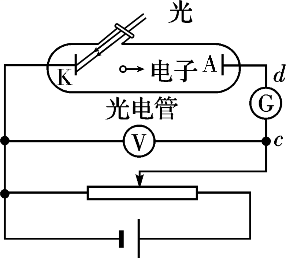
\includegraphics[width=1.30208in,height=1.17917in]{media/image468.png}\end{center}
A.a光的频率一定大于b光的频率

B.只增加a光的强度可使通过电流计G的电流增大

C.增加b光的强度可能使电流计G的指针发生偏转

D.用a光照射光电管阴极K时通过电流计G的电流是由d到c

E.用a光照射时,增大光电管两端的电压时,流过G的电流可能不变
\newpage
\subsection{光电效应的图象分析}
\begin{longtable}[]{@{}m{2.5cm}m{3cm}m{7cm}@{}}
\toprule
图象名称
&
图线形状
&
由图线直接(间接)
得到的物理量\tabularnewline
\midrule
\endhead
最大初动能Ek与入射光频率ν的关系图线
&
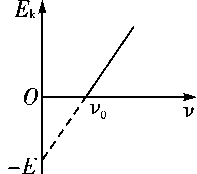
\includegraphics[width=0.89653in,height=0.79236in]{media/image469.png}\strut

&
\ding{172}极限频率:ν0

\ding{173}逸出功:W0=\textbar-E\textbar=E

\ding{174}普朗克常量:图线的斜率k=h
\tabularnewline
遏止电压Uc与入射光频率ν的关系图线
&
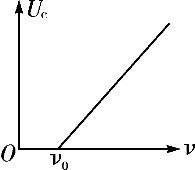
\includegraphics[width=0.88681in,height=0.77361in]{media/image470.png}\strut
& 
\ding{172}截止(极限)频率:ν0

\ding{173}遏止电压Uc:随入射光频率的增大而增大

\ding{174}普朗克常量:h=ke (k为斜率,e为电子电量)
\tabularnewline
频率相同、光强不同时,光电流与电压的关系
&
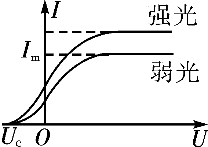
\includegraphics[width=0.94306in,height=0.67014in]{media/image471.png}\strut

&
\ding{172}遏止电压:Uc

\ding{173}饱和光电流:Im(电流的最大值)

\ding{174}最大初动能:Ekm=eUc
\tabularnewline
频率不同、光强相同时,光电流与电压的关系
&
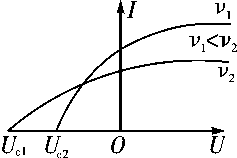
\includegraphics[width=1.07569in,height=0.71667in]{media/image472.png}\strut
&
\ding{172}遏止电压:Uc1、Uc2

\ding{173}饱和光电流:电流最大值

\ding{174}最大初动能:$E_{k1}=eUc1$,$E_{k2}=eUc2$
\tabularnewline
\bottomrule
\end{longtable}

\begin{center}
  
\includegraphics[width=0.70764in,height=0.12292in]{media/image37.png}
\end{center}
\begin{center}
  \textbf{定量分析光电效应时应抓住的三个关系式}
\end{center}

(1)爱因斯坦光电效应方程:Ek=hν-W0.

(2)最大初动能与遏止电压的关系:Ek=eUc.

(3)逸出功与极限频率、极限波长λc的关系:W0=hνc=h.

{[}例2{]}(2017·湖北武汉模拟)从1907年起,美国物理学家密立根开始以精湛的技术测量光电效应中几个重要的物理量.他通过如图所示的实验装置测量某金属的遏止电压Uc与入射光频率ν,作出Uc-ν的图象,由此算出普朗克常量h,并与普朗克根据黑体辐射测出的h相比较,以检验爱因斯坦方程的正确性.图中频率ν1、ν2,遏止电压Uc1、Uc2及电子的电荷量e均为已知,求:

\begin{center}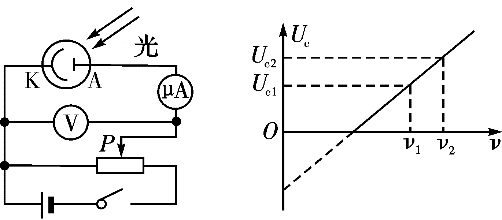
\includegraphics[width=2.28333in,height=1in]{media/image473.png}\end{center}
(1)普朗克常量h;

(2)该金属的截止频率ν0.

{[}思维导引{]} (1)明确最大初动能Ek与入射光的频率ν的关系;

(2)明确最大初动能与遏止电压Uc的关系;

(3)理解Uc-ν图线与横轴交点的物理意义.

答案 (1)() (2)
\newpage
\subsection{光的波粒二象性 物质波}

光既有波动性,又有粒子性,两者不是孤立的,而是有机的统一体,其表现规律为

(1)从数量上看:个别光子的作用效果往往表现为粒子性;大量光子的作用效果往往表现为波动性.

(2)从频率上看:频率越低波动性越显著,越容易看到光的干涉和衍射现象;频率越高粒子性越显著,贯穿本领越强,越不容易看到光的干涉和衍射现象.

(3)从传播与作用上看:光在传播过程中往往表现出波动性;在与物质发生作用时往往表现为粒子性.

(4)波动性与粒子性的统一:由光子的能量E=hν、光子的动量表达式p=也可以看出,光的波动性和粒子性并不矛盾,表示粒子性的能量和动量的计算式中都含有表示波的特征的物理量------频率ν和波长λ.

(5)理解光的波粒二象性时不可把光当成宏观概念中的波,也不可把光当成宏观概念中的粒子.

\begin{center}
\includegraphics[width=0.70764in,height=0.12292in]{media/image13.png}\end{center}
\begin{center}
  \textbf{波粒二象性的深入理解}
\end{center}

(1)虽然平时看到宏观物体运动时,看不出其波动性,但也有一个波长与之对应.例如飞行子弹的波长约为10-34
m.

(2)波粒二象性是微观粒子的特殊规律,一切微观粒子都存在波动性;宏观物体也存在波动性,只是波长太小,难以观测.

(3)德布罗意波也是概率波,衍射图样中的亮圆是电子落点概率大的地方,但概率的大小受波动规律的支配.

{[}例3{]}用很弱的光做双缝干涉实验,把入射光减弱到可以认为光源和感光胶片之间不可能同时有两个光子存在,如图所示是不同数量的光子照射到感光胶片上得到的照片.这些照片说明( D )

\begin{center}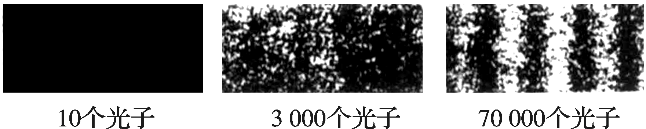
\includegraphics[width=2.93403in,height=0.58472in]{media/image474.png}\end{center}
A.光只有粒子性没有波动性

B.光只有波动性没有粒子性

C.少量光子的运动显示波动性,大量光子的运动显示粒子性

D.少量光子的运动显示粒子性,大量光子的运动显示波动性

解析 由这些照片可以看出,少量光子的运动显示粒子性,大量光子的运动呈现出波动性,故选项D正确.
\newpage
\section{原子结构与原子核}

1.原子核式结构

(1)电子的发现:英国物理学家\_\_汤姆孙\_\_发现了电子.

(2)$\alpha$粒子散射实验:1909~1911年,英国物理学家\_\_卢瑟福\_\_和他的助手进行了用$\alpha$粒子轰击金箔的实验,实验发现\_\_绝大多数\_\_$\alpha$粒子穿过金箔后基本上仍沿原来的方向前进,但有\_\_少数\_\_$\alpha$粒子发生了大角度偏转,\_\_极少数\_\_$\alpha$粒子偏转的角度甚至大于$90^\circ$,也就是说它们几乎被``撞''了回来.如图所示.

\begin{center}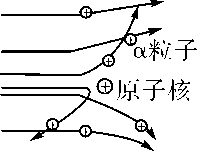
\includegraphics[width=0.89653in,height=0.68889in]{media/image477.png}\end{center}

(3)原子的核式结构模型:在原子中心有一个很小的核,原子全部的\_\_正电荷\_\_和几乎全部\_\_质量\_\_都集中在核里,带负电的电子在核外空间绕核旋转.

2.氢原子光谱

(1)光谱分析

利用元素的特征谱线(线状谱)分析和确定物质的组成成分.

(2)氢原子光谱的实验规律

巴耳末系是氢光谱在可见光区的谱线,其波长公式=R(-)
.(n=3,4,5,\ldots,R是里德伯常量,R=1.10\ding{54}107 m-1)

(3)玻尔模型

\ding{172}玻尔的三条假设

a.能量量子化:原子只能处于一系列\_\_不连续\_\_状态中,在这些状态中原子是稳定的,电子虽然绕核运动,但并不向外辐射能量,这些状态叫做\_\_定态\_\_.

对氢原子满足:En=E1,其中E1=-13.6 eV.

b.轨道量子化:原子的\_\_能量状态\_\_跟电子不同的运行\_\_轨道\_\_相对应.原子的能量状态是不连续的,因此电子运动的可能轨道的分布也是不连续的.

对氢原子满足:rn=n2r1,其中r1=0.53\ding{54}10-10 m.

c.能级跃迁:原子从一种定态(设能量为E2)跃迁到另一种定态(设能量为E1)时,它\_\_辐射或吸收\_\_一定频率的光子,光子的能量由这两种定态的能量差决定,即hν=E2-E1.

\ding{173}氢原子能级图:如图所示.

\begin{center}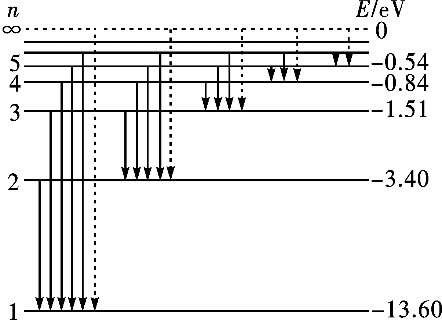
\includegraphics[width=2.00972in,height=1.45278in]{media/image478.png}\end{center}
\newpage
3.原子核

(1)天然放射现象的发现

1896年,\_\_贝可勒尔\_\_在铀矿石中发现未知的射线,把这些射线称为$\alpha$射线、$\beta$射线、γ射线,这就是天然放射现象的发现.天然放射现象的发现,说明原子核\_\_具有复杂结构\_\_.

(2)三种射线的比较

\begin{longtable}[]{@{}m{2cm}m{2cm}m{3cm}m{2.5cm}@{}}
\toprule
种类 & $\alpha$射线 & $\beta$射线 & γ射线\tabularnewline
\midrule
\endhead
组成 & 高速氦核流 & 高速电子流 & 光子流\tabularnewline
带电荷量 & 2e & -e & 0\tabularnewline
质量 & 4mp & & 静止质量为零\tabularnewline
在电磁场中 & 偏转 & 与$\alpha$射线反向偏转 & 不偏转\tabularnewline
穿透本领 & & &\tabularnewline
电离作用 & & &\tabularnewline
\bottomrule
\end{longtable}

(3)原子核的衰变

\ding{172}衰变

原子核由于自发地放出某种粒子而转化为新核的变化.

\ding{173}衰变规律

a.$\alpha$衰变:X$\rightarrow$Y+He,实质:2H+2n$\rightarrow$He.

b.$\beta$衰变:X$\rightarrow$Y+e,实质:n$\rightarrow$H+e.

\ding{174}半衰期

a.定义:放射性元素衰变有一定的速率,我们把放射性元素的原子核有半数发生衰变需要的时间叫半衰期,用τ表示.

b.公式:m=m0().

c.特点:半衰期τ由该元素的原子核内部本身的因素决定,跟原子所处的物理状态(如压强、温度等)或化学状态(如单质、化合物等)无关.另外,半衰期仅是对大量原子核的统计规律.比如研究200个铀的原子核经过一个半衰期后还剩多少个铀的原子核是没有意义的.

4.核能

(1)核力

核子间的作用力.核力是短程强力,作用范围在1.5\ding{54}10-15
m之内,只在\_\_相邻\_\_的核子间发生作用.

(2)核能

\_\_核子\_\_结合为原子核时释放的能量或原子核分解为核子时吸收的能量,叫做原子核的\_\_结合\_\_能,亦称核能.

(3)质能方程、质量亏损

爱因斯坦质能方程E=\_\_mc2\_\_,原子核的质量必然比组成它的核子的质量和要小,这就是质量亏损$\Delta$m.由质量亏损可求出释放的核能$\Delta$E=\_\_$\Delta$mc2\_\_.

(4)重核的裂变与轻核的聚变

\ding{172}裂变

重核分裂成质量较小的核的反应.如:U+n$\rightarrow$Xe+Sr+10n. 

\ding{173}聚变

轻核结合成质量较大的核的反应.如:H+H$\rightarrow$He+n.
\newpage
\subsection{能级图与氢原子的跃迁}

1.能级图中相关量意义的说明

\begin{longtable}[]{@{}m{5cm}m{7cm}@{}}
\toprule
相关量 & 意义\tabularnewline
\midrule
\endhead
能级图中的横线 & 表示氢原子可能的能量状态------定态\tabularnewline
横线左端的数字``1,2,3\ldots'' & 表示量子数\tabularnewline
横线右端的数字``-13.6,-3.4\ldots'' & 表示氢原子的能量\tabularnewline
相邻横线间的距离 &
表示相邻的能量差,量子数越大相邻的能量差越小,距离越小\tabularnewline
带箭头的竖线 &
表示原子由较高能级向较低能级跃迁,原子跃迁的条件为hν=Em-En\tabularnewline
\bottomrule
\end{longtable}

氢原子的能级图如图所示.

\begin{center}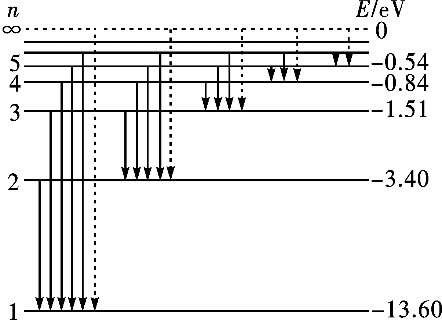
\includegraphics[width=2.00972in,height=1.45278in]{media/image478.png}\end{center}

2.两类能级跃迁

(1)自发跃迁:高能级$\rightarrow$低能级,释放能量,发出光子.

光子的频率ν==.

(2)受激跃迁:低能级$\rightarrow$高能级,吸收能量.

\ding{172}光照(吸收光子):光子的能量必须恰等于能级差$hν\neq E$;

\ding{173}碰撞、加热等:只要入射粒子能量大于或等于能级差即可,E外≥$\Delta$E;

\ding{174}大于电离能的光子被吸收,将原子电离.

\begin{center}
\includegraphics[width=0.70764in,height=0.12292in]{media/image13.png}\end{center}
\begin{center}
    \textbf{谱线条数的确定方法}
\end{center}

(1)一个氢原子跃迁发出可能的光谱线条数最多为(n-1).

(2)一群氢原子跃迁发出可能的光谱线条数的两种求解方法.

\ding{172}用数学中的组合知识求解:N=C=();

\ding{173}利用能级图求解:在氢原子能级图中将氢原子跃迁的各种可能情况一一画出,然后相加.
\newpage
\subsection{原子核的衰变 半衰期}

1.$\alpha$衰变、$\beta$衰变的比较

\begin{longtable}[]{@{}m{2cm}m{5cm}m{5cm}@{}}
\toprule
衰变类型 & $\alpha$衰变 & $\beta$衰变\tabularnewline
\midrule
\endhead
衰变方程 & X―$\rightarrow$Y+He & X$\rightarrow$Y+e\tabularnewline
衰变实质 & 2个质子和2个中子结合成一个整体射出 &
1个中子转化为1个质子和1个电子\tabularnewline
& 2H+2n―$\rightarrow$He & n―$\rightarrow$H+e\tabularnewline
\begin{minipage}[t]{0.30\columnwidth}\raggedright
匀强磁场中

轨迹形状\strut
\end{minipage} & \begin{minipage}[t]{0.30\columnwidth}\raggedright
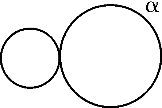
\includegraphics[width=0.73611in,height=0.49028in]{media/image480.png}\strut
\end{minipage} & \begin{minipage}[t]{0.30\columnwidth}\raggedright
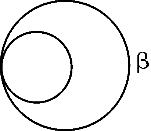
\includegraphics[width=0.68889in,height=0.59444in]{media/image481.png}\strut
\end{minipage}\tabularnewline
衰变规律 & 电荷数守恒、质量数守恒、动量守恒 &\tabularnewline
\bottomrule
\end{longtable}

2.确定$\alpha$、$\beta$衰变次数的两种方法

方法1:确定衰变次数的方法是依据两个守恒规律,设放射性元素X经过n次$\alpha$衰变和m次$\beta$衰变后,变成稳定的新元素Y,则表示该核反应的方程为:X―$\rightarrow$Y+nHe+me.

根据质量数守恒和电荷数守恒可列方程

A=A'+4n,Z=Z'+2n-m

由以上两式联立解得

n=,m=+Z'-Z

由此可见,确定衰变次数可归结为求解一个二元一次方程组.

方法2:因为$\beta$衰变对质量数无影响,可先由质量数的改变确定$\alpha$衰变的次数,然后再根据衰变规律确定$\beta$衰变的次数.

3.半衰期

(1)公式:N余=N原(),m余=m原().

(2)影响因素:放射性元素衰变的快慢是由原子核内部自身因素决定的,跟原子所处的物理状态(如温度、压强)或化学状态(如单质、化合物)无关.

{[}例2{]}(2017·宁夏银川质检)U经过m次$\alpha$衰变和n次$\beta$衰变,变成Pb,则( B )

A.m=7,n=3 B.m=7,n=4

C.m=14,n=9 D.m=14,n=18

解析 根据题意知核反应方程U$\rightarrow$Pb+mHe+ne,根据电荷数守恒和质量数守恒可得235=207+4m,92=82+2m-n.联立解得m=7,n=4,选项B正确.

{[}例3{]}(2018·四川宜宾模拟)碘131核不稳定,会发生$\beta$衰变,其半衰期为8天.

(1)碘131核的衰变方程:I$\rightarrow$\_\_54X+e\_\_.(衰变后的元素用X表示)

(2)经过\_\_16\_\_天有75\%的碘131核发生了衰变.

解析 (1)根据质量数和电荷数守恒可知衰变方程为I$\rightarrow$X+e.

(2)每经1个半衰期,有半数原子核发生衰变,经2个半衰期将剩余的原子核,即有75\%的碘131核发生衰变,故经过的时间为16天.
\newpage
\subsection{核反应类型与核反应方程}

1.核反应的四种类型

\begin{longtable}[]{@{}m{1cm}m{1cm}m{2cm}m{5cm}@{}}
\toprule
\multicolumn{2}{l}{类型}& 可控性 & 核反应方程 \tabularnewline
\midrule
\endhead
\multirow{2}{2cm}{衰变}
&
$\alpha$衰变
&
自发
&
U―$\rightarrow$Th+He\strut
\tabularnewline
& $\beta$衰变 & 自发 & Th$\rightarrow$Pa+e\tabularnewline
\multicolumn{2}{l}{人工转变}
&
\multirow{2}{2cm}{人工控制}    
&
N+He―$\rightarrow$O+H

(卢瑟福发现质子)

He+Be―$\rightarrow$C+n

(查德威克发现中子)

Al+He―$\rightarrow$P+n

P―$\rightarrow$Si+e

(约里奥·居里夫妇发现放射

性同位素,同时发现正电子)
\tabularnewline
\multicolumn{2}{l}{重核裂变}
& &
U+n―$\rightarrow$Ba+Kr+3n

U+n―$\rightarrow$Xe+Sr+10n
\tabularnewline
\multicolumn{2}{l}{轻核聚变}
& 很难控制 & H+H―$\rightarrow$He+n \tabularnewline
\bottomrule
\end{longtable}

2.核反应方程式的书写

(1)熟记常见基本粒子的符号是正确书写核反应方程的基础.如质子(H)、中子(n)、$\alpha$粒子(He)、$\beta$粒子(e)、正电子(e)、氘核(H)、氚核(H)等.

(2)核反应过程一般都是不可逆的,所以核反应方程只能用单向箭头连接并表示反应方向,不能用等号连接.

(3)核反应的生成物一定要以实验为基础,不能凭空只依据两个守恒规律杜撰出生成物来写核反应方程.

(4)核反应过程中质量数守恒,核电荷数守恒.

{[}例4{]}在下列四个核反应中,x表示中子的是哪些?\_\_BCD\_\_.

在以下核反应中哪些属于原子核的人工转变?\_\_AB\_\_.

A.N+He$\rightarrow$O+x B.Al+He$\rightarrow$P+x

C.H+H$\rightarrow$He+x D.U+x$\rightarrow$Sr+Xe+10x

解析 不管什么类型的核反应,都遵守电荷数守恒和质量数守恒,由以上两个守恒规则,可以分别计算出A、B、C、D中x的质量数和电荷数,分别为A中x,B中x,C中x,D中x,所以x表示中子的是B、C、D;关于人工转变问题,首先应明确核反应的特点:有粒子作``炮弹''轰击作为``靶''的原子核,并且能在实验室中进行,因此人工核转变的有A、B,C叫轻核聚变,D叫重核裂变.
\newpage
\subsection{核能的计算}

1.质能方程的理解

(1)一定的能量和一定的质量相联系,物体的总能量和它的质量成正比,即E=mc2.

方程的含义是:物体具有的能量与它的质量之间存在简单的正比关系,物体的能量增大,质量也增大;物体的能量减少,质量也减少.

(2)核子在结合成原子核时出现质量亏损$\Delta$m,释放的能量为$\Delta E\neq mc2$.

(3)原子核分解成核子时要吸收一定的能量,相应的质量增加$\Delta$m,吸收的能量为$\Delta E\neq mc2$.

2.核能释放的两种途径的理解

中等大小的原子核的比结合能最大,这些核最稳定.

(1)使较重的核分裂成中等大小的核.

(2)较小的核结合成中等大小的核,核子的比结合能都会增加,都可以释放能量.

3.计算核能的几种方法

(1)根据$\Delta E\neq mc2$计算,计算时$\Delta$m的单位是``kg'',c的单位是``m/s'',$\Delta$E的单位是``J''.

(2)根据$\Delta E\neq m$\ding{54}931.5 MeV计算.因1原子质量单位``u''相当于931.5
MeV的能量,所以计算时$\Delta$m的单位是``u'',$\Delta$E的单位是``MeV''.

(3)根据核子比结合能来计算核能

原子核的结合能=核子比结合能\ding{54}核子数.

{[}例5{]}一个静止的铀核U(原子质量为232.037 2
u)放出一个$\alpha$粒子(原子质量为4.002 6 u)后衰变成钍核Th(原子质量为228.0287
u).(已知:原子质量单位1 u=1.67\ding{54}10-27 kg,1 u相当于931.5 MeV)

(1)写出核衰变反应方程;

(2)算出该核衰变反应中释放出的核能;

(3)假设反应中释放出的核能全部转化为钍核和$\alpha$粒子的动能,则钍核获得的动能有多大?

解析 (1)92U$\rightarrow$90Th+He.

(2)质量亏损$\Delta$m=mU-mTh-m$\alpha$=0.005 9 u,

$\Delta E\neq mc2=0.0059$\ding{54}931.5 MeV=5.496 MeV.

(3)系统动量守恒,钍核和$\alpha$粒子的动量大小相等,即

pTh-p$\alpha$=0,EkTh=,Ek$\alpha$=, EkTh+Ek$\alpha \neq E$;

所以钍核获得的动能EkTh=\ding{54}$\Delta$E=\ding{54}$\Delta$E=0.095 MeV

答案 (1) U$\rightarrow$Th+He

(2)5.496 MeV (3)0.095 MeV
